\documentclass{article}

\usepackage{graphicx}
\usepackage{tikz}
\usepackage{tikzsymbols}
\usetikzlibrary{calc,patterns,shapes.geometric}
\pagestyle{empty}
\usepackage[margin=0pt]{geometry}
\geometry{papersize={14in,12in}}

\def\centerarc[#1](#2)(#3:#4:#5){\draw[#1] ($(#2)+({#5*cos(#3)},{#5*sin(#3)})$) arc (#3:#4:#5);}

\begin{document}
	\begin{figure}
		\centering
		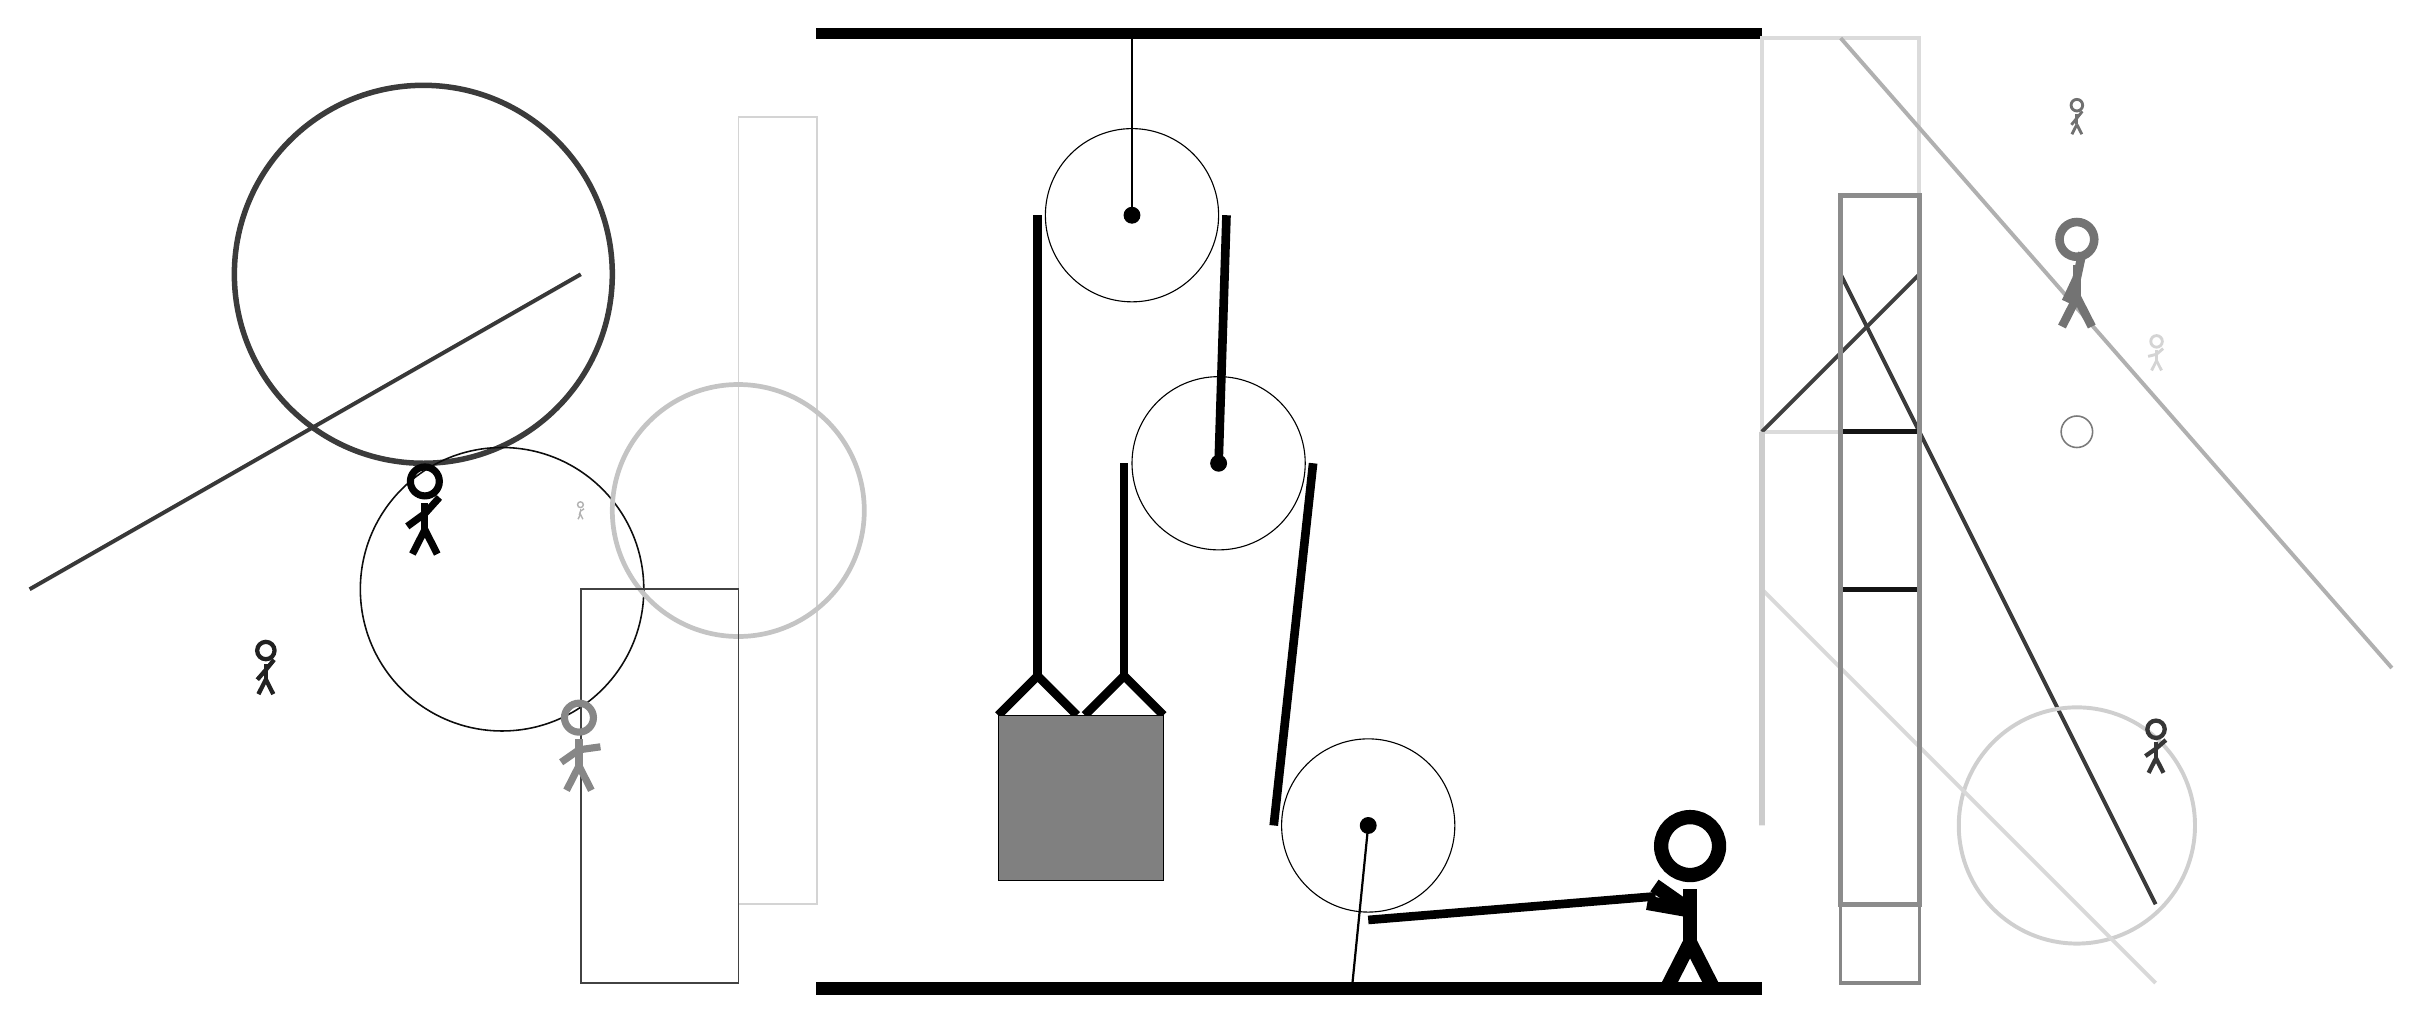
\begin{tikzpicture}
			%%%%% START %%%%%
			
			\draw[fill=black] (-2, 9) rectangle (10, 9.125);
			
			\draw (2, 6.75) circle (1.1);
			\draw[fill=black] (2, 6.75) circle (0.1);
			\draw[thick] (2, 6.75) -- (2, 9);
			
			\draw (3.1, 3.6) circle (1.1);
			\draw[fill=black] (3.1, 3.6) circle (0.1);
			
			\draw (5, -1) circle (1.1);
			\draw[fill=black] (5, -1) circle (0.1);
			\draw[thick] (5, -1) -- (4.8, -3);
			
			\draw[line width=0.3mm, color=black!28] (11, 2) rectangle (11, -2);
			
			\draw[line width=0.2mm, color=black!99] (12, 8) rectangle (12, 9);
			\node[line width=0.5mm, color=black!56] at (14, 8) {\Strichmaxerl[2][51][51]};
			\draw[line width=0.5mm, color=black!77](11, 6) -- (15, -2);
			
			\node[line width=0.4mm, color=black!87] at (-9, 1) {\Strichmaxerl[3][49][51]};
			\draw[line width=0.5mm, color=black!14] (12, 9) rectangle (10, 4);
			\draw [line width=0.5mm, color=black!19](14, -1) circle (1.5);
			\draw[line width=0.5mm, color=black!31](11, 9) -- (18, 1);
			\draw [line width=0.2mm, color=black!52](14, 4) circle (0.2);
			\draw[line width=0.5mm, color=black!75](12, 6) -- (10, 4);
			\draw[line width=0.5mm, color=black!15](10, 2) -- (15, -3);
			\draw [line width=0.7mm, color=black!77](-7, 6) circle (2.4);
			\draw[line width=0.4mm, color=black!47] (12, -2) rectangle (11, -3);
			\draw [line width=0.2mm, color=black!95](-6, 2) circle (1.8);
			\node[line width=0.4mm, color=black!55] at (14, 6) {\Strichmaxerl[6][65][78]};
			\node[line width=0.3mm, color=black!79] at (15, 0) {\Strichmaxerl[3][35][41]};
			
			\node[line width=0.2mm, color=black!30] at (-5, 3) {\Strichmaxerl[1][74][33]};
			\draw[line width=0.2mm, color=black!17] (-3, -2) rectangle (-2, 8);
			\draw[line width=0.5mm, color=black!78](-5, 6) -- (-12, 2);
			
			\draw [line width=0.6mm, color=black!23](-3, 3) circle (1.6);
			\draw[line width=0.2mm, color=black!74] (-3, -3) rectangle (-5, 2);
			\node[line width=0.3mm, color=black!17] at (15, 5) {\Strichmaxerl[2][14][41]};
			
			\draw[line width=0.6mm, color=black!92] (12, 2) rectangle (11, 4);
			\draw[line width=0.7mm, color=black!20] (10, -1) rectangle (10, 4);
			\node[line width=0.5mm, color=black!47] at (-5, 0) {\Strichmaxerl[5][35][8]};
			
			\node[line width=0.6mm, color=black!99] at (-7, 3) {\Strichmaxerl[5][36][48]};
			
			\draw[line width=0.6mm, color=black!45] (11, -2) rectangle (12, 7);
			
			\draw[line width = 1.1mm]  (0.3, 0.4) -- (0.8, 0.9) -- (1.3, 0.4);
			\draw[line width = 1.1mm]  (1.4, 0.4) -- (1.9, 0.9) -- (2.4, 0.4);
			\draw[fill=black!50] (0.3, 0.4) rectangle (2.4, -1.7);
			
			\draw[line width = 1.1mm] (0.8, 6.75) -- (0.8, 0.9);
			\centerarc[line width = 1.1mm](2, 6.75)(0:180:1.2000000000000002);
			\draw[line width = 1.1mm] (3.2, 6.75) -- (3.1, 3.6);
			\draw[line width = 1.1mm] (1.9, 3.6) -- (1.9, 0.9);
			\centerarc[line width = 1.1mm](3.1, 3.6)(0:180:1.2000000000000002);
			\draw[line width = 1.1mm] (4.3, 3.6) -- (3.8, -1);
			\centerarc[line width = 1.1mm](5, -1)(180:270:1.2000000000000002);
			\draw[line width = 1.1mm] (5, -2.2) -- (8.65, -1.9);
			
			\node at (9, -2) {\Strichmaxerl[10][-35][170]};
			
			\draw[fill=black] (-2, -3) rectangle (10, -3.15);
			
			%%%%% END %%%%%
		\end{tikzpicture}
	\end{figure}	
\end{document}